\subsection{Using Stars to Sequentially Scan the Huge Graph at Most Once}\label{sec:match_star}
Because of the intrinsic poor locality of graphs,
tree-based algorithms would incur incredible random disk accesses when jumping between the vertices scattered among the disk.
Therefore, a join based matching algorithm is more suitable for real world problems.
However, to \emph{choose a proper join unit that can avoid random disk accesses and minimize the intermediate results as well} is still a hard problem.
Perhaps the most intuitive way is to decompose the original pattern graph into a series of edges.
However, lots of useless intermediate results would be generated by doing so.
Consider the diamond pattern graph in Figure~\ref{img:pattern_graph},
many intermediate results would be generated if they were matched in Figure~\ref{img:celebrity_star},
however, they are all pointless since there is no such a graph that could match the original diamond pattern.
To solve this problem, more complex structures such as frequent subgraphs, multi-hop edges could be used,
however, as Sun et al\@. have stated before,
these methods require complex index that has super-linear space and time complexity~\cite{DBLP:journals/pvldb/SunWWSL12}, and are not very suitable for solving real world property graph matching problems.

Recall the vertex-centric property graph storage model that we discussed previously,
which provides two efficient iterators that can scan the vertices (via \textsc{VertexIter}) and neighbors (via \textsc{NeighborIter}) sequentially (Section~\ref{sec:storage_iterators}),
if the matching process only requires neighborhood link information,
random disk accesses could then be avoided.
Based on this observation, we make a balance by using stars as our basic matching unit.
As is shown in Figure~\ref{img:pattern_graph}, a star graph contains a root vertex and some neighbors connected to the root.
The star pattern can then be matched within a sequential disk scan based on our vertex-centric storage model:
1\@. Select the domain of interest using the global index,
2\@. iterate through the relevant vertices by the \textsc{VertexIter},
3\@. and for each visited vertex, use the \textsc{NeighborIter} to check the neighbors to determine whether the star would be matched.
Besides, a star contains far more structural information then an edge,
which means the matching results of a star have a predictable smaller size.
Moreover, we made further contributions to keep the matching results even smaller (Section~\ref{sec:match_compress} and Section~\ref{sec:match_optimize}).

Some authors also adopt star-like structures as their basic matching unit~\cite{DBLP:journals/pvldb/SunWWSL12,DBLP:journals/pvldb/LaiQLC15},
however, our contribution takes further steps in three different ways:
\begin{enumerate}[noitemsep,leftmargin=*]
\item In order to make a practical graph matching engine, we adopt the property graph model (Section~\ref{sec:background}) rather than the simple graph model ubiquitous among academical paper.
  A simple graph can be viewed as a special case of a property graph,
  which ignores the labels, multi-edges, or even the direction of edges.
  However, real world applications of simple graphs are very limited because of the information they dropped out.
  It is not easy to make a simple graph matching algorithm to solve the property graph matching problem.
  For one thing, it is a hard engineering problem, because the traditional underlying graph storage method is not suitable for property graphs (Section~\ref{sec:storage}).
  For another, many existing work rely on the perfect isotropic properties of a simple graph to operate and optimize their algorithms~\cite{DBLP:journals/pvldb/SunWWSL12,DBLP:conf/sigmod/HanLL13,DBLP:journals/pvldb/QiaoZC17}.
\item We developed a novel pattern decomposition algorithm that is able to preserve as much matching information as possible, whereas the existing decomposition methods may lose information and result in gigantic useless intermediate results.
  Consider the pattern graph in Figure~\ref{img:star_decomposition},
  suppose that $u_1$, $u_2$ and $u_3$ are selected as the roots,
  existing decomposition method would result in three stars with 3, 2 and 1 neighbor\@(s)
  by consecutively selecting and removing vertices from the original pattern.
  However, many useful matching information are lost by doing so,
  e.g., the third ``star'' is just an edge, which would generate enormous unnecessary matching results whereas every edge in the data graph would match it but only a part of them could match the original pattern graph.
  In contrast, our approach (Algorithm~\ref{alg:decompose_stars}) would keep all the neighborhood matching information as is shown in the bottom of Figure~\ref{img:star_decomposition}, which could then reduce unnecessary intermediate results significantly (Section~\ref{sec:experiments}).
  Like previous work~\cite{DBLP:journals/pvldb/SunWWSL12}, we also use a heuristic function to select a join order, which is defined as $ f(u) = \frac{\deg(u) + |\psi(u)|}{\operatorname{freq}(u.label)} $, i.e.,
  we prefer to select vertex with bigger degree (more early filters) and less label frequency (smaller intermediate matching results) first.
  $|\psi(u)|$ is the number of local constraints of $u$, which will be discussed further in Section~\ref{sec:match_optimize}.
  The root candidate set $R$ is used to select a connected vertex cover,
  which could then be joined efficiently (Section~\ref{sec:match_join}).
  The key feature of the algorithm is to remove selected vertex in a copy $p'$ of the pattern and always keeps the original useful information in $p$, and thus, the intermediate results of our star could be much smaller.
  \begin{figure}[ht]
    \centering
    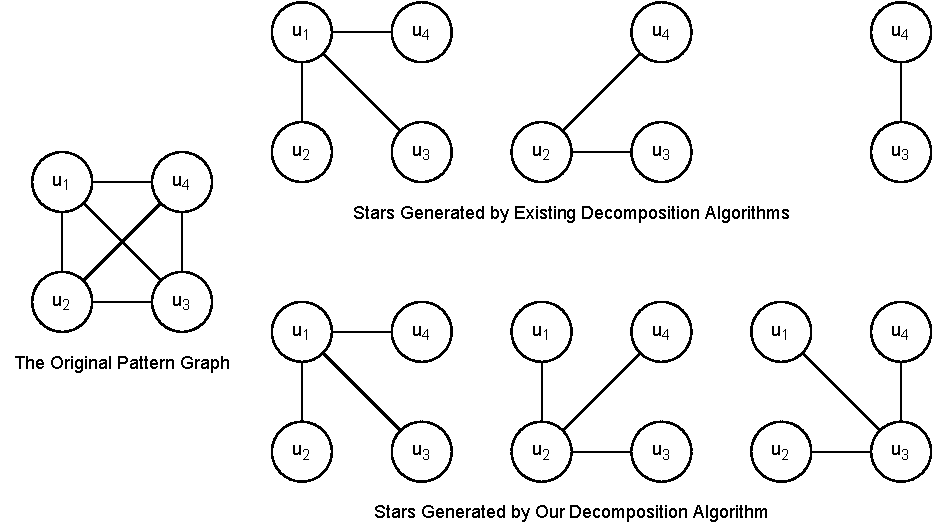
\includegraphics[width=0.48\textwidth]{img/star_decomposition.pdf}
    \caption{Stars decomposed from the same pattern graph using different algorithms.}\label{img:star_decomposition}
  \end{figure}
\item As the real-world billion node graphs are so large that it is preferable to scan it only once in a streaming style when solving a property graph matching problem.
  However, it is not a simple task because multiple stars has to be matched in a single sequential scan,
  the context switch cost and the intermediate result write cost must be minimized.
  For the context switch cost, it is strongly coupled with the underlying storage method of the data graph.
  Thanks to the elegant design of our vertex-centric storage model,
  which is able to match stars in a sequential run given a root label,
  we could group the stars with the same root label together and match them at the same time when iterating through \textsc{VertexIter}.
  For the matching result write cost, we developed a compression algorithm for star's matching results that could be wrote sequentially (Section~\ref{sec:match_compress}).
  As a result, we could scan the huge data graph only once and all the I/Os are sequential.
\end{enumerate}
\begin{algorithm}[ht]
  \caption{Star Decomposition}\label{alg:decompose_stars}
  \SetKwFunction{DecomposeStars}{\textsc{DecomposeStars}}
  \SetKwFunction{Peek}{\textsc{Peek}}
  \SetKwFunction{Star}{\textsc{Star}}
  \SetKwFunction{RemoveVertex}{\textsc{RemoveVertex}}
  \Input{The pattern graph $p$}
  \Output{A sequence of stars with a specific order}
  \Fn{\DecomposeStars{$p$}}{
    $results \leftarrow \emptyset$\;
    $p' \leftarrow p$\;
    $R \leftarrow \{\max_{u \in V(p)}f(u)\}$\;
    \While{$R \neq \emptyset$}{
      $root \leftarrow \max_{u \in R}f(u)$\;
      $R \leftarrow R \setminus \{ root \}$\;
      $R \leftarrow R \cup \{ leaf \mid leaf \text{ is adjacent to } root \text{ in } p'\}$\;
      \RemoveVertex{$p'$, $root$}\;
      $R \leftarrow R \setminus \{ u \mid u \in p' \land \deg{u} = 0 \}$\;
      $results \leftarrow results \cup \{$ \Star{$p$, $root$} $\}$\;
    }
    \Return{$results$}
  }
\end{algorithm}
